
\documentclass[]{report}

\usepackage{ifthen}
\usepackage[utf8]{inputenc}
\usepackage{lmodern}
\usepackage[T1]{fontenc}
\usepackage{graphicx}
\usepackage{epstopdf} % Permet d'utiliser des images eps
\usepackage{hyperref}
\usepackage[left=1cm, right=2.5cm, top=2.5cm, bottom=4.5cm]{geometry}
\usepackage{fancyhdr}
\usepackage{changepage}
\usepackage{titletoc}
\usepackage{lipsum} % Package à enlever (Lorem ipsum)
\usepackage{makecell}
\usepackage{tocloft}

\usepackage{subcaption}

% Packages pour le calendrier
\usepackage{tikz}
\usetikzlibrary[positioning]
\usetikzlibrary{patterns}

%-----------------------------------------------------------------%
% DÉFINITIONS
%-----------------------------------------------------------------%
\renewcommand*\contentsname{Table des matières}

\renewcommand\cftaftertoctitle{\par\noindent\hrulefill\par\vskip-2.3em}

\setlength{\cftbeforetoctitleskip}{0pt}

\titlecontents
    {section}
    [3.8em]
    {}
    {\contentslabel{2.3em}}
    {\hspace*{-2.3em}}
    {\titlerule*[1pc]{}\contentspage}

\titlecontents
    {subsection}
    [3.8em]
    {}
    {\contentslabel{2.3em}}
    {\hspace*{-2.3em}}
    {\titlerule*[1pc]{}\contentspage}

%-----------------------------------------------------------------%
% HAUTS ET BAS DE PAGES
%-----------------------------------------------------------------%
\pagestyle{fancy}

\fancyhf{}
\lhead{\includegraphics[width=3.68cm]{Figures/folie-logo.png} \qquad
CAMP DE JOUR FOLIE TECHNIQUE 2019}

\rfoot{\thepage}
\lfoot{© Folie Technique, [2019]. Tous droits réservés.}

%-----------------------------------------------------------------%
% DOCUMENT
%-----------------------------------------------------------------%
\begin{document}

%-----------------------------------------------------------------%
% Page titre
%-----------------------------------------------------------------%
\newgeometry{margin=3.5cm}

\begin{titlepage}
\begin{center}

\Huge{Camp de jour Folie Technique
\\
Été 2019}
\\[3.25 in]
\huge \textbf{Informatique Avancée}
\\
\Large Thématique 14-17 ans
\\[3.25 in]
POLYTECHNIQUE MONTRÉAL
\\
Par Fermion \& Béryllium

\end{center}
\end{titlepage}

\restoregeometry

%-----------------------------------------------------------------%
% Table des matières
%-----------------------------------------------------------------%
\headheight = 79.32524pt

\begin{adjustwidth}{1.5cm}{0cm}
\tableofcontents\thispagestyle{fancy}
\end{adjustwidth}

\newpage

%-----------------------------------------------------------------%
% Introduction
%-----------------------------------------------------------------%
\begin{adjustwidth}{1.5cm}{0cm}

\subsection*{\Large{Introduction}}
\addcontentsline{toc}{subsection}{Introduction}
\vspace{-5mm}\makebox[0.917\textwidth]{\hrulefill}\vspace{3mm}

La semaine \textit{Informatique Avancé} introduira aux jeunes le langage C++ qui est un langage fondamental de l'informatique. Ils apprenderont comment manipuler des variables, des fonctions ainsi que le système de classe offert par C++. Ils apprenderont comment 
toutes les notions abordés au cours de la semaine peuvent être utilisés simultanement pour créer des programmes intéractifs et amusants.
\\[6pt]
Il est pris pour aquis que les jeunes inscrits ont déjà fait de la programmation, peu importe le langage\footnote{Excepté le «langage» HTML qui n'est pas un langage de programmation.}, mais sans toutefois avoir fait de la programmation de haut-niveau. Par exemple, un jeune ayant participé à une semaine \textit{Informatique} auparavant serait parfaitement en mesure de participer à cette semaine. 
%-----------------------------------------------------------------%
% Horaire de la semaine
%-----------------------------------------------------------------%
\subsection*{\Large{Horaire de la semaine}}
\addcontentsline{toc}{subsection}{Horaire de la semaine}
\vspace{-5mm}\makebox[0.917\textwidth]{\hrulefill}\vspace{3mm}

\begin{center}
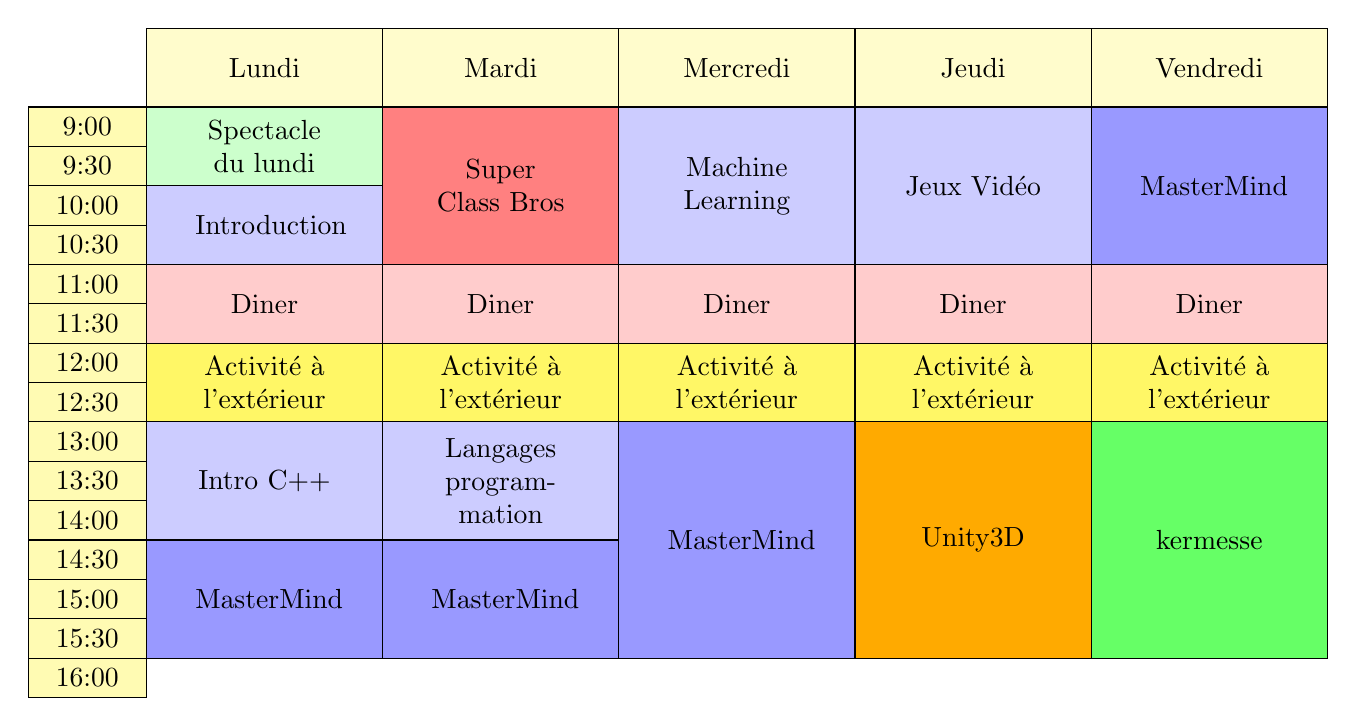
\begin{tikzpicture}[x=3 cm, y=-1cm, node distance=0 cm,outer sep = 0pt]

% Style des jours
\tikzstyle{day}=[draw, rectangle,  minimum height=1cm, minimum width=3 cm, fill=yellow!20,anchor=south west]

% Style des heures
\tikzstyle{hour}=[draw, rectangle, minimum height=0.5 cm, minimum width=1.5 cm, fill=yellow!30,anchor=north east]

% Positions des jours et des heures 
\node[day] (lundi) at (1,8) {Lundi};
\node[day] (mardi) [right = of lundi] {Mardi};
\node[day] (mercredi) [right = of mardi] {Mercredi};
\node[day] (jeudi) [right = of mercredi] {Jeudi};
\node[day] (vendredi) [right = of jeudi] {Vendredi};
\node[hour] (9) at (1,8) {9:00};
\node[hour] (9-30)  [below = of 9]      {9:30};
\node[hour] (10)    [below= of 9-30]    {10:00};
\node[hour] (10-30) [below = of 10]     {10:30};
\node[hour] (11)    [below = of 10-30]  {11:00};
\node[hour] (11-30) [below = of 11]     {11:30};
\node[hour] (12)    [below = of 11-30]  {12:00};
\node[hour] (12-30) [below = of 12]     {12:30};
\node[hour] (13)    [below = of 12-30]  {13:00};
\node[hour] (13-30) [below = of 13]     {13:30};
\node[hour] (14)    [below = of 13-30]  {14:00};
\node[hour] (14-30) [below = of 14]     {14:30};
\node[hour] (15)    [below = of 14-30]  {15:00};
\node[hour] (15-30) [below = of 15]     {15:30};
\node[hour] (16)    [below = of 15-30]  {16:00};

% Définition des grandeurs des cases selon les durées
\tikzstyle{hours}=[rectangle,draw, minimum width=3 cm, anchor=north west,text centered,text width=5 em]
\tikzstyle{0:30}=[hours,minimum height=0.5cm]
\tikzstyle{1:00}=[hours,minimum height=1cm]
\tikzstyle{1:30}=[hours,minimum height=1.5cm]
\tikzstyle{2:00}=[hours,minimum height=2cm]
\tikzstyle{2:30}=[hours,minimum height=2.5cm]
\tikzstyle{3:00}=[hours,minimum height=3cm]

% Définitions des activités (durées et couleurs)
\tikzstyle{spectacleLundi}    = [1:00,fill=green!20]
\tikzstyle{diner}             = [1:00,fill=red!20]
\tikzstyle{activiteExterieur} = [1:00,fill=yellow!60]
\tikzstyle{kermesse}          = [3:00,fill=green!60]

% Présentations
\tikzstyle{introduction}		= [1:00, fill = blue!20]
\tikzstyle{introC++}			= [1:30, fill = blue!20]
\tikzstyle{AI++}				= [2:00, fill = blue!20]
\tikzstyle{langages}			= [1:30, fill = blue!20]
\tikzstyle{jeuxvideo}		= [2:00, fill = blue!20]

% Activités
\tikzstyle{mastermindfull}	= [3:00, fill = blue!40]
\tikzstyle{masterminddeux}	= [2:00, fill = blue!40]
\tikzstyle{mastermindhalf}	= [1:30, fill = blue!40]
\tikzstyle{mastermindhour}	= [1:00, fill = blue!40]
\tikzstyle{superclassbros}	= [2:00, fill = red!50]

% Sortie
\tikzstyle{sortie}			= [3:00, fill = {rgb:red,1;green,0;yellow,2}]

% Position des événements
% Lundi
\node[spectacleLundi] at (1,8) {Spectacle du lundi};
\node[introduction] at (1, 9) {Introduction};
\node[diner] at (1,10) {Diner};
\node[activiteExterieur] at (1,11) {Activité à l'extérieur};
\node[introC++] (1) at (1, 12) {Intro C++};
\node[mastermindhalf] (14-30) [below = of 1] {MasterMind};

% Mardi
\node[superclassbros] at (2, 8) {Super Class Bros};
\node[diner] at (2,10) {Diner};
\node[activiteExterieur] at (2,11) {Activité à l'extérieur};
\node[langages] (2) at (2, 12) {Langages programmation};
\node[mastermindhalf] (14-30) [below = of 2] {MasterMind};

% Mercredi
\node[AI++] at (3, 8) {Machine Learning};
\node[diner] at (3,10) {Diner};
\node[activiteExterieur] at (3,11) {Activité à l'extérieur};
\node[mastermindfull] at (3, 12) {MasterMind};

% Jeudi
\node[jeuxvideo] at (4, 8) {Jeux Vidéo};
\node[diner] at (4,10) {Diner};
\node[activiteExterieur] at (4,11) {Activité à l'extérieur};
\node[sortie] at (4, 12) {Unity3D};

% Vendredi
\node[masterminddeux] at (5, 8) {MasterMind};
\node[diner] at (5,10) {Diner};
\node[activiteExterieur] at (5,11) {Activité à l'extérieur};
\node[kermesse] at (5,12) {kermesse};

\end{tikzpicture}
\end{center}

%-----------------------------------------------------------------%
% Conseils
%-----------------------------------------------------------------%
%\subsection*{\Large{Conseils}}
%\addcontentsline{toc}{subsection}{Conseils}
%\vspace{-5mm}\makebox[0.917\textwidth]{\hrulefill}\vspace{3mm}

\newpage
%-----------------------------------------------------------------%
% Activité
%-----------------------------------------------------------------%
\section*{\centering\underline{Hello World!}}
\addcontentsline{toc}{section}{Hello World!}

\subsection*{\Large{Sommaire}}
\vspace{-5mm}\makebox[0.917\textwidth]{\hrulefill}\vspace{3mm}

L'activité \textit{Hello World} servira d'activité d'introduction à la programmation en C++ ainsi que de vérifier le niveau de connaissance des jeunes. Elle introduit des notions de base qui serviront à l'actité \textit{MasterMind}. Les jeunes devront faire un programme intéractif qui leur demande des informations sur eux (\textit{exemple: nom, âge, etc.)} et devra être capable de bien fonctionner malgré des erreurs que l'utilisateur pourrait faire.

\vspace{1cm}

\begin{center}
\begin{tabular}{ccc}\cline{1-1} \cline{3-3}
\multicolumn{1}{|c|}{\makecell{\textbf{\underline{Durée approximative}} \\ 1h}} & & \multicolumn{1}{|c|}{\makecell{\textbf{\underline{Coût approximatif par jeune}} \\ 0.00\$}}\\ \cline{1-1} \cline{3-3}
\\ \cline{1-1} \cline{3-3}
\multicolumn{1}{|c|}{\makecell{\textbf{\underline{Niveau de difficulté (1 à 5)}} \\ 2}} & & \multicolumn{1}{|c|}{\makecell{\textbf{\underline{Groupe d’âge}} \\ 14-17 ans}}\\ \cline{1-1} \cline{3-3}
\\ \cline{1-1} \cline{3-3}
\multicolumn{1}{|c|}{\makecell{\textbf{\underline{Matériel}} \\ aucun}} & & \multicolumn{1}{|c|}{\makecell{\textbf{\underline{Notions abordées}} \\ - Variables\\ - Fonctions\\ - Boucles}} \\ \cline{1-1} \cline{3-3}
\end{tabular}
\end{center}

\subsection*{\Large{Théorie}}
\vspace{-5mm}\makebox[0.917\textwidth]{\hrulefill}\vspace{3mm}

En programmation, une \textbf{variable} est simplement une espace mémoire alloué qui est associé à un symbole donné par le programmeur. Une variable, en C++, n'est pas obligée de contenir une valeur, mais son type doit toujours être précisé! La valeur de la variable peut être \textit{librement} modifiée à tout moment dans le programme, d'où le nom \textit{variable}.
\\

Tel que mentionné, une variable à ce qu'on appelle un \textbf{type} qui est tout simplement la nature de la valeur contenue à l'intérieur de la variable. Les nombres entiers et décimaux sont de type \textit{int} et \textit{float}, les caractères simples sont des \textit{char} tandis que les chaines de caractères sont des \textit{string} et il y a le type \textit{boolean} qui peut seulement prendre 0 ou 1 comme valeur. La nature du type influence le rôle que la variable peut avoir dans le programme; les \textit{string} ne sont pas utilisés pour compter, mais bien pour stocker des phrases ou autres chaines de caratères.
\\

Les \textbf{boucles}, en programmation, sont utilisées pour effectuer une certaine tâche plusieurs fois sans devoir à copier-coller des sections de code et ainsi le programme inutilement. De plus, le nombre de fois qu'une tâche doit être répéter peut être inconnu lors de la compilation ou même varier. En C++, les deux boucles que l'on peut utilisées sont les boucles \textit{for} et \textit{while}; habituellment, la boucle \textit{for} est employée lorsque le nombre d'itération est «connu» tandis que la boucle \textit{while} est utilisée lorsque le nombre d'itération dépend d'une certaine condition.\\ 

Peu importe le type de boucle utilisée, le fonctionnement reste le même: avant d'entrer à l'intérieur de la boucle, une certaine condition -préciser par le programmeur- détermine si oui ou non la boucle peut se répéter. Dans le cas oùla condition est respectée, on entre dans le corps de la boucle et le code s'ytrouvant se fait exécuter. Lorsque l'exécution du coprs est fait, on vérifie si la condition est toujours respectée; si c'est le cas on entre à nouveau dans la boucle, sinon on continue dans le programme en ignorant le corps de la boucle.\\

Voici un exemple de chaque type de boucle:
\begin{figure}[!h]
	\centering
	\includegraphics[scale=0.5]{Figures/boucles.png}
	\caption{Démonstration de boucles \texttt{FOR} et \texttt{WHILE}}
	\label{hw:fig:boucles}
\end{figure}

Les \textbf{fonctions}, en programmation, sont utilisées pour exécuter une certaine procédure en appelant la fonction aux endroits désirés; tout comme les boucles, l'utilisation de fonctions permet d'écrire du code à un seul endroit plutôt que de recopier la procédure à chaque fois qu'il faut l'exécuter. Une fonction peut avoir, ou non, des arguments qui sont tout simplement les variables qui seront utilisées par la fonctions, exactement comme une fonction en mathématique. Lorsqu'on programme en C++, les fonctions ne peuvent retourner qu'une seule valeur et le type de la valeur retournée doit être le même que le type de la fonction. Donc si la fonction retourne un nombre entier, son type devrait être \textit{int}. Une fonction peut toutefois rien retourner dans le programme et son type serait alors \textit{void}. Lorsqu'une fonction est utilisée à l'intérieur d'un programme, disons que notre fonction se nomme \textit{print}, on écrit simplement le nom de la fonction suivie des arguments qui seront utilisés entre parenthèses. Voici un exemple d'une fonction:

\begin{figure}[!h]
	\centering
	\includegraphics[scale=0.5]{Figures/FONCTIONS.png}
	\caption{Exemple de fonction}
	\label{hw:fig:fonctions}
\end{figure}

Toutes les notions sont abordées à l'intérieur de la présentation \textit{Introdution à C++} avec des exemples plus détailés.
\subsection*{\Large{Manipulation}}
\vspace{-5mm}\makebox[0.917\textwidth]{\hrulefill}\vspace{3mm}

Commencer l'activité avec la présentation \textit{Introduction à C++} qui introduit des notions de bases du langages. Pour chaque nouvelle notion abordée, assurez-vous que les jeunes comprennent bien avant de passer à la prochaine. La présentation parlera des bons comportements à avoir lorsqu'on programme, des variables, des types, des boucles ainsi que des fonctions.
\\

Lorsque la présentation est terminé, crééer un nouveau projet avec les jeunes nommé \textit{Hello World!} et expliquer leur le but de l'activité. Continuier ensuite par leur montrer comment utiliser les fonctions \textit{cout} et \textit{cin} du langage pour qu'ils sachent comment créer une intéraction entre l'utilisateur et la console (le programme). 
\\

Les jeunes devront maintenant essayer de programmer le code qui fait les tâches suivantes:
\begin{enumerate}
	\item Message d'introdution\\
	\item Demande à l'utilisateur son nom\\
	\item Demande à l'utilisateur son age\\
	\item Message personnalisé avec le nom et l'age\\
	\item Pécise à l'utilisatuer s'il est majeur ou non\\
\end{enumerate}
Le tout devra être à l'intérieur d'une boucle et la console demande à la fin si l'utilisateur veut quitter le programme; si il répond oui le programme se termine sinon il se répère du début.

\subsection*{\Large{Présentation suggérée}}
\vspace{-5mm}\makebox[0.917\textwidth]{\hrulefill}\vspace{3mm}

Il est fortement recommendé de faire l'activité avec la présentation \textit{Introduction à C++} puisque toutes les notions utilisées y sont présentées.

\newpage
\subsection*{\Large{Code de référence}}
\vspace{-5mm}\makebox[0.917\textwidth]{\hrulefill}\vspace{3mm}
\begin{figure}[h]
	\centering
	\includegraphics[scale=0.5]{Figures/helloWorld.png}
	\caption{Exemple d'un code pour HelloWorld!}
	\label{hw:fig:code}
\end{figure}
\newpage
%-----------------------------------------------------------------%
% Activité
%-----------------------------------------------------------------%
\section*{\centering\underline{MasterMind}}
\addcontentsline{toc}{section}{MasterMind}

\subsection*{\Large{Sommaire}}
\vspace{-5mm}\makebox[0.917\textwidth]{\hrulefill}\vspace{3mm}

Cette activité est l'activité principale de la semaine durant laquelle les jeunes devront reproduire le jeu \textit{Mastermind} à l'aide d'un programme qu'ils écriront.  Chaque jeune devra écrire le code du jeu, mais ils peuvent tout de même communiquer entre eux pour s'aider. L'activité se déroulera durant toute la semaine pour construire itérativement le code; d'autres activités/présentations introduiront de nouveaux concepts qui seront par la suite utilisés pour améliorer leur programme. Le but de l'activité est de familiariser les jeunes avec les concepts vus durant la semaine ainsi que d'améliorer leur compétence à abstraire et segmenter un problème pour le reproduire à l'aide d'un programme informatique.

\vspace{1cm}

\begin{center}
\begin{tabular}{ccc}\cline{1-1} \cline{3-3}
\multicolumn{1}{|c|}{\makecell{\textbf{\underline{Durée approximative}} \\ 12h}} & & \multicolumn{1}{|c|}{\makecell{\textbf{\underline{Coût approximatif par jeune}} \\ 0.00\$}}\\ \cline{1-1} \cline{3-3}
\\ \cline{1-1} \cline{3-3}
\multicolumn{1}{|c|}{\makecell{\textbf{\underline{Niveau de difficulté (1 à 5)}} \\ 4}} & & \multicolumn{1}{|c|}{\makecell{\textbf{\underline{Groupe d’âge}} \\ 14-17 ans}}\\ \cline{1-1} \cline{3-3}
\\ \cline{1-1} \cline{3-3}
\multicolumn{1}{|c|}{\makecell{\textbf{\underline{Matériel}} \\ - a}} & & \multicolumn{1}{|c|}{\makecell{\textbf{\underline{Notions abordées}} \\ - a}} \\ \cline{1-1} \cline{3-3}
\end{tabular}
\end{center}

\subsection*{\Large{Théorie}}
\vspace{-5mm}\makebox[0.917\textwidth]{\hrulefill}\vspace{3mm}

La théorie de cette activité provient des autres présentations faites durant la semaine; cette activité n'introduit aucune nouvelle notion aux jeunes, mais les fusionne en une seule activité. Les jeunes apprendront donc à utiliser tous les concepts vus durant la semaine et comment les utiliser dans un seul programme.


\subsection*{\Large{Déroulement}}
\vspace{-5mm}\makebox[0.917\textwidth]{\hrulefill}\vspace{3mm}

La première étape de l'activité est de présenter aux jeunes le vrai jeu \textit{Mastermind} et de leur expliquer comment on y joue. Les règlements se trouvent plus loin dans cette section. Assurez-vous que les jeunes ont bien compris les règlements ainsi que les étapes d'une partie de \textit{Mastermind}, car ils auront beaucoup de difficulté par la suite sinon. Essayer ensuite de leur faire décortiquer les mécanismes du jeu et comment les joueurs interagissent lors d'une partie; n'hésiter pas à les aider pour compléter cette partie puisqu'elle est cruciale pour le reste de l'activité.
\\

Lorsque le jeu est bien compris par tous, les jeunes peuvent maintenant commencer à faire le code. La première étape à réaliser est de créer le projet avec les jeunes. Nommez le projet \textit{Mastermind} et le premier fichier \textit{Source.cpp}. Créer ensuite une classe \textit{MasterMindGame} qui ajoutera au projet deux fichiers portant le même nom avec les extensions \textit{.cpp} et \textit{.h}.
\\

Les jeunes programmeront le code entièrement par eux-même; aucun code troué ne leur sera fourni; le programme sera donc construit itérativement en implémentant les conceptes abordés par les autres activités et modifiant le code existant en conséquence des ajouts apportés. L'animateur doit toutfois être capable de les aider au besoin. Votre rôle sera donc d'introduire les notions utiles ainsi que d'aider les jeunes à les implémenter dans leur code. 

\subsection*{\Large{Étapes du programme}}
\vspace{-5mm}\makebox[0.917\textwidth]{\hrulefill}\vspace{3mm}
Les 

\textbf{$1^e$ itération interaction joueur-console}\\
Le première étape du code serait d'implementer une première version du systeme permettant l'intéraction joueur-console. Ce systeme est simplement une boucle qui demande au joueur d'entrer son choix, le stock dans une certaine variable et puis l'affiche à la console. À chaque itération, le nombre d'essaie actuel du joueur ainsi que le nombre d'essaie maximum doivent être affichés. La condition d'arrêt de la boucle est simplement lorsque la valeur de l'essaie actuelle est plus grande que la valeur maximale. Demander d'abord aux jeunes d'utiliser la fonction \texttt{cin} et montrer leur pourquoi il serait préférable d'utiliser la fonction \texttt{getline()}.\\[6pt]
\textit{Petit rappel:} La fonction \textit{cin} sépare le input à chaque espacement fait et stock les mots dans différents \textit{buffer} ce qui cause certains problème pour le jeu que l'on veut faire.\\

\textbf{$2^e$ itération initialisation de la classe}\\
La seconde étape consiste à implémenter une première version de la classe \textit{MasterMindGame} et d'utiliser ses méthodes pour automatiser l'attribution des valeurs à certaines variables. Dans le \textit{header file} de la classe, il faut ajouter les attributs \textit{codeCache, codeLongueur, essaie, essaieMax} comme attributs \textit{privés} et les méthodes \textit{getters GetCodeLongueur, GetEssaie et GetEssaieMax} ainsi que la méthode \textit{Reset} comme méthodes publiques. Repréciser aux jeunes la différence entre les propriétés privé et publique et pourquoi on choisi de mettre, par exemple, l'attribut \textit{codeCache} privé.\\

\textbf{$3^e$ itération choix du joueur}\\
La troisième itération consiste à implémenter une fonction (à l'intérieur du fichier \textit{Source.cpp}) pour s'assurer que le choix du jouer est valide. La fonction devra afficher le nombre d'essaie du joueur et lui demander son choix. Le choix sera directement utilisé par la méthode \textit{GetStatusChoix} de la classe \textit{MasterMindGame}; la méthode devra retourné le status \textit{OK} si le choix est valide ou \textit{NOT\_SAME\_LENGTH} ou \textit{NOT\_VALID\_CARACTER} selon le cas. La méthode \textit{GetStatusChoix} devra donc être capable de déterminer si la longueur du choix fait est la même que celle du code caché et si le choix contient uniquement des caractères valides. Si le choix n'est pas valide, un message lui précisant son erreur devrait apparaître à la console pour qu'il puisse faire un meilleur choix à son prochain essai. Presque l'entierté de la fonction se trouve à l'intérieur d'une boucle dont l'unique manière de sortir est lorsque le choix fait est valide, ou autrement dit, lorsque le statu retourné par la méthode est \textit{OK}. Le choix fait est alors retourné par la fonction.
\\

\textbf{$4^e$ itération}\\
La quatrième itération du code implémente une manière de mettre à jour le score du joueur selon le choix qu'il vient de faire. Tout le code qui sera ajouté par cette étape se retrouve presqu'entièrement à l'intérieur de la classe \textit{MasterMindGame}. Pour ce faire il faut ajouter la méthode \textit{UpdateScore} qui accepte comme argument le choix du choix sous forme de \textit{string} et retourne simplement le score du joueur. Pour déterminer le score du joueur, il suffit simplement de faire un boucle chaque caractère du choix et à l'intérieur de cette boucle, de faire une seconde boucle sur chaque caractère du code caché. Pour chaque pair de caractère, il est facile de déterminer s'il s'agit d'un \textit{blanc} ou d'un \textit{noir} et ainsi mettre à jour le score. C'est également à l'intérieur de cette méthode que l'on vérifie si le joueur à gagné.  Ceci est la manière \textit{naïve} et comporte un petit \textit{bug} qui n'est aps nuissible; vous pouvez demander aux jeunes d'essayer de régler ce problème lorsqu'ils auront fini. 

%\subsection*{\Large{Présentation suggérée}}
%\vspace{-5mm}\makebox[0.917\textwidth]{\hrulefill}\vspace{3mm}

%Tel que mentionné, le but de cette activité n'est pas d'introduire de nouvelles notions aux jeunes, mais plutôt de leur montrer comment bien utiliser les notions vus durant la semaine en un seul programmme fonctionnel. Il n'y a donc pas de présentation suggérée. Par contre, n'hésitez pas à réutiliser les présentations vues précédemment.

\newpage
%-----------------------------------------------------------------%
% Activité
%-----------------------------------------------------------------%
\section*{\centering\underline{SuperClassBros}}
\addcontentsline{toc}{section}{SuperClassBros}

\subsection*{\Large{Sommaire}}
\vspace{-5mm}\makebox[0.917\textwidth]{\hrulefill}\vspace{3mm}

Durant cette activité, les jeunes devront reconstruire la hiérarchie de classes du jeu \textit{Super Mario Bros} à l'aide d'une image qui sera présentée à l'écran. L'activité peut se faire en équipe, ou seul si un jeune le souhaite, et sa durée est approximativement 30 minutes; le temps alloué peut facilement être modifié pour s'adapter à l'intérêt des jeunes. 
\\ 

Le but de cette activité est de familiariser les jeunes avec les concepts d'héritage, de méthodes et d'attributs d'une classe et d'interaction entre classes. Cette activité développera l'aptitude des jeunes à reconnaître ce que peut être une classe, à visualiser la hiérarchie d'un groupe de classe -en remarquant la similitude entre les classes- ainsi que de déterminer quels méthodes et attributs une classe pourrait posséder.

\vspace{1cm}

\begin{center}
\begin{tabular}{ccc}\cline{1-1} \cline{3-3}
\multicolumn{1}{|c|}{\makecell{\textbf{\underline{Durée approximative}} \\ 1h30min}} & & \multicolumn{1}{|c|}{\makecell{\textbf{\underline{Coût approximatif par jeune}} \\ 0\$}}\\ \cline{1-1} \cline{3-3}
\\ \cline{1-1} \cline{3-3}
\multicolumn{1}{|c|}{\makecell{\textbf{\underline{Niveau de difficulté (1 à 5)}} \\ 3}} & & \multicolumn{1}{|c|}{\makecell{\textbf{\underline{Groupe d’âge}} \\ 14-17 ans}}\\ \cline{1-1} \cline{3-3}
\\ \cline{1-1} \cline{3-3}
\multicolumn{1}{|c|}{\makecell{\textbf{\underline{Matériel}} \\ - Présentation \textit{SuperClassBros} \\ - Papier \\ - Crayon }} & & \multicolumn{1}{|c|}{\makecell{\textbf{\underline{Notions abordées}} \\ - Attibuts \\ - Méthodes \\ - Héritage \\ - Class}} \\ \cline{1-1} \cline{3-3}
\end{tabular}
\end{center}

\subsection*{\Large{Théorie}}
\vspace{-5mm}\makebox[0.917\textwidth]{\hrulefill}\vspace{3mm}

En informatique, une classe est une structure de donnée permettant l'encapsulation de fonctions et de variables à l'intérieur d'un objet et est utilisée dans la programmation orientée objet qui favorise l'interaction entre plusieurs classes. Une classe peut également avoir des classes «filles» qui héritent de toutes les méthodes et attributs de leur «mères» et doivent en posséder davantage; les classes filles sont moins générales que leur classe mère et leurs méthodes sont plus précises.
\\

Par exemple, soit les classes \textit{Personne}, \textit{Élève}, \textit{Personnel}, \textit{Enseignant} tel que la classe \textit{Personne} a les attributs suivants: \textit{prénom}, \textit{nom}, \textit{date\_de\_naissance}. Cette classe pourrait être la classe mère des classes \textit{Élève} et \textit{Personnel}; on ajouterait alors à la classe \textit{Élève} d'autres attributs tel que \textit{programme}, \textit{moyenne}, etc. et à la classe \textit{Personnel} les attributs \textit{ancienneté}, \textit{salaire}, etc. Puis, la classe \textit{Enseignant} serait la classe fille de \textit{Personnel} et on lui ajouterait les attributs \textit{domaine\_de\_recherche}, \textit{cours}, etc.
\\

Tel que mentionné, une classe est une strucutre de données qui permet d'encapsuler des variables ainsi que des fonctions; les variables et fonctions attachées à une classe sont respectivement nommées \textbf{attributs} et \textbf{méthodes}. Si une fonction peut être vue comme une procédure qui est executé lorsqu'elle est appelé, alors une classe est une \textit{blueprint} qui construit un ceertain objet avec certains attributs et que l'on peut manipuler par la suite à l'aide des méthodes de la classe. Plusieurs objets d'une même classe peuvent re instanciés en même temps et chaque objet se comportera indépendamment des autres. Par exemple, pour un jeu vidéo, une classe \textit{Joueur} peut être utiliser autant de fois qu'il y a de personne jouant au jeu et chacune de ces personnes contrôlera une entité différente. Les attributs et méthodes d'une classe peuvent soient être \textit{publique} ou \textit{privée}; un attribut/fonction \textit{publique} peut directement être utilisé ou modifié à \textit{l'exterieur} de la classe en utilisant le «.» tandis qu'un attribut/fonction \textit{privé} n'est accessible ou modifiable qu'à l'intérieur de la classe. En reprenant l'exemple de la classe \textit{Joueur}, une attribut pourrait être la vie du joueur et un tel attribut ne devrait pas être modifié hors de la classe, mais uniquement en utilisant des méthodes publiques de la classe. On protège donc certains attributs/méthodes en les \textit{taggant} comme privés.

\subsection*{\Large{Matériel}}
\vspace{-5mm}\makebox[0.917\textwidth]{\hrulefill}\vspace{3mm}

Simplement du papiers et des crayons pour que les jeunes puissent écrire leur hiérarchie plus facilement. Oridnateur également nécéssaire.

\subsection*{\Large{Déroulement}}
\vspace{-5mm}\makebox[0.917\textwidth]{\hrulefill}\vspace{3mm}

Débutez l'activité avec la théorie sur les classes présente dans la présentation \textit{SuperClassBros}. Assurez-vous que les jeunes comprennent bien ce qu'est une classe, la différences entre ce qu'est un attributs et une méthodes ainsi que ce qu'est une hiérarchie. Lorsque les jeunes sont prêts, commencez l'activité.
\\

Présentez à l'écran l'image du jeu \textit{Super Mario bros} et expliquez interactivement avec les jeunes les éléments présents sur l'image ainsi qu'une petite explication du jeu, si nécéssaire. Puis, passez à la présentation qui contient les mots clés et laissez les jeunes faire la hiérarchie! Votre rôle n'est pas de leur donner les réponses, mais plutôt de les guider si jamais ils sont perdus. Précisez également aux jeunes qu'il n'y a pas de mauvaises réponces, mais que certaines hiérarchies vont simplifier la construction du jeu et que d'autres vont compliquer les choses.
\\

Lorsque les jeunes ont terminé, construiser avec eux la hiérarchie en utilisant leur réponses et modifier-les aux besoins. Tel que mentionné il n'y a pas vraiment de mauvaise réponse, mais certaine compliqueront la hiérarchie et il serait préférable de ne pas les utiliser. Lorsque la hiérarchie est complétée, et si les jeunes semble toujours intéressés, ajouter des nouveaux éléments au jeu et demander aux jeunes à quel endroit dans la hiérarchie chaque élément devrait se trouver. Par exemple, si vous ajouter le personnage \textit{Princess Fermion}, on devrait retrouver cet élément sous la classe \textit{Entité} et selon le cas, \textit{Enemie} ou \textit{NPC}/\textit{Joueur}. Cette activité devrait facilement montrer aux jeunes la force d'utiliser une hiérarchie de classe et à quel pointe cela facilite l'ajout de nouveaux éléments.

\subsection*{\Large{Présentation suggérée}}
\vspace{-5mm}\makebox[0.917\textwidth]{\hrulefill}\vspace{3mm}

Seule la présentation \textit{SuperClassBros} est nécéssaire; elle contient la théorie sur les classes ainsi que l'activité elle-même.



\end{adjustwidth}
\end{document}
\newpage
%-----------------------------------------------------------------%
% Activité
%-----------------------------------------------------------------%

\section*{\centering\underline{“Nom de l’activité”}}
\addcontentsline{toc}{section}{“Nom de l’activité”}

\subsection*{\Large{Sommaire}}
\vspace{-5mm}\makebox[0.917\textwidth]{\hrulefill}\vspace{3mm}

\lipsum[1]

\vspace{1cm}

\begin{center}
\begin{tabular}{ccc}\cline{1-1} \cline{3-3}
\multicolumn{1}{|c|}{\makecell{\textbf{\underline{Durée approximative}} \\ h}} & & \multicolumn{1}{|c|}{\makecell{\textbf{\underline{Coût approximatif par jeune}} \\ \$}}\\ \cline{1-1} \cline{3-3}
\\ \cline{1-1} \cline{3-3}
\multicolumn{1}{|c|}{\makecell{\textbf{\underline{Niveau de difficulté (1 à 5)}} \\ 3}} & & \multicolumn{1}{|c|}{\makecell{\textbf{\underline{Groupe d’âge}} \\ ans}}\\ \cline{1-1} \cline{3-3}
\\ \cline{1-1} \cline{3-3}
\multicolumn{1}{|c|}{\makecell{\textbf{\underline{Matériel}} \\ - a \\ - b}} & & \multicolumn{1}{|c|}{\makecell{\textbf{\underline{Notions abordées}} \\ - a \\ - b}} \\ \cline{1-1} \cline{3-3}
\end{tabular}
\end{center}

\subsection*{\Large{Théorie}}
\vspace{-5mm}\makebox[0.917\textwidth]{\hrulefill}\vspace{3mm}

\lipsum[1]

\subsection*{\Large{Matériel}}
\vspace{-5mm}\makebox[0.917\textwidth]{\hrulefill}\vspace{3mm}

\lipsum[1]

\subsection*{\Large{Manipulation}}
\vspace{-5mm}\makebox[0.917\textwidth]{\hrulefill}\vspace{3mm}

\lipsum[1]

\subsection*{\Large{Présentation suggérée}}
\vspace{-5mm}\makebox[0.917\textwidth]{\hrulefill}\vspace{3mm}

\lipsum[1]

\subsection*{\Large{Sources d’erreur}}
\vspace{-5mm}\makebox[0.917\textwidth]{\hrulefill}\vspace{3mm}

\lipsum[1]

